% Fig. 3.14 -- once the truncated piece is divided by the probability of the
%   stretch it sits on, it is a legitimate pdf again.
% Source: mathstatch3.tex lines 1558-1590.
%
% The manuscript keeps the shape of its previous picture and raises the peak
% from 2 to 3, i.e. multiplies by 1.5, drawing the curve on 1.6 <= x <= 4.4
% only; it shades the whole of the block underneath, drops the same two
% dashed boundaries, and labels the curve f_X(x|a<X<b).
%
% The web version carries over the density of truncated-range.tex (Fig. 3.13)
% and divides it by the probability of the block, so the multiplier is not
% chosen but computed:
%   f_X(x) = 0.3989423 e^{-(x-3)^2/2},  a = 2.0,  b = 4.4
%   P(a<X<b) = 0.7605876
%   f_X(x|a<X<b) = f_X(x)/P(a<X<b) = 0.5245182 e^{-(x-3)^2/2},  a < x < b
% The lift is therefore 1/0.7605876 = 1.3147721, and the shaded block of this
% figure encloses area 1 where the shaded block of Fig. 3.13 encloses
% 0.7605876.
%
% Drawing scale x = 1.05cm, y = 6.4cm, both the same as Fig. 3.13, and the
% invisible \path across the foot is the same as well, so that the two
% drawings are exactly as wide as each other and therefore render at one
% scale whatever width the column has.  Heights: peak 3.35692cm,
% f_X(a|a<X<b) = 2.03607cm, f_X(b|a<X<b) = 1.25989cm; the peak of Fig. 3.13
% stands at 2.55323cm, and 3.35692/2.55323 is the 1.3147721 above.
%
% Deviations from the manuscript picture:
%
% 1. The curve label sits above the peak rather than off to the upper right,
%    where the manuscript puts it.  Off to the right it would set the right
%    edge of the drawing, and the drawing would no longer be as wide as
%    Fig. 3.13, which is what keeps the two peaks comparable.
%
% 2. \DeclareMathSizes{10}{10}{9}{8} raises the math script sizes from the
%    default 7pt/5pt, as CH2_FIGURE_SPECS.md 1.3 requires wherever \sssig
%    appears.  Native size 221.82 x 135.906 pt (drawing 7.65cm wide, shared
%    with Fig. 3.13).  A mark of S pt shows at
%    S x 0.99626 x <display width> / 221.82 px, so at the 350px phone width
%    of a topic-figure--wide in body text
%        10pt text 15.72px, 9pt scripts 14.15px, 8pt scriptscripts 12.58px
%    and at the 620px desktop width 27.85 / 25.06 / 22.28px.
\documentclass[tikz,border=2pt]{standalone}
\usepackage{amsmath}
\usepackage{amssymb}
\usepackage{xcolor}
\usetikzlibrary{arrows.meta}
\newcommand{\sssig}{\scriptscriptstyle}
\DeclareMathSizes{10}{10}{9}{8}

\definecolor{journalink}{HTML}{1F1C18}
\definecolor{journalmuted}{HTML}{8A7F72}
\definecolor{journalaccent}{HTML}{9C2D2D}

\begin{document}
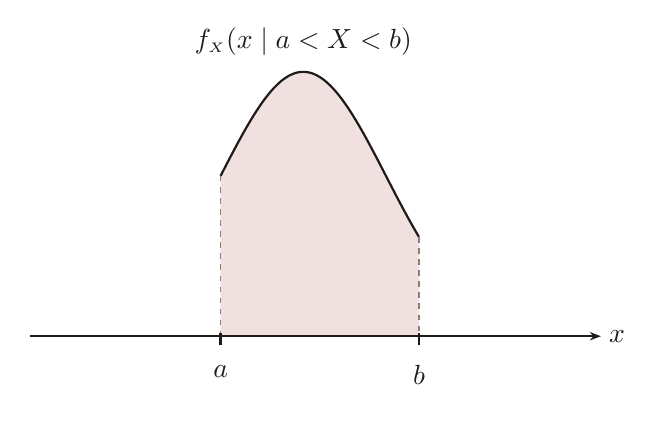
\begin{tikzpicture}[
  x=1.05cm,
  y=6.4cm,
  every node/.style={font=\normalsize, journalink},
  axis/.style={journalink, line width=0.8pt, -{Stealth[length=4pt]}},
  tick/.style={journalink, line width=0.8pt},
  curve/.style={journalink, line width=0.8pt},
  guide/.style={journalmuted, line width=0.5pt, dash pattern=on 2pt off 2pt},
  region/.style={journalaccent, fill opacity=0.15}
]
  % ---- left edge, right edge and floor, shared with Fig. 3.13 ----------
  \path (-0.35cm,-0.70cm) -- (7.30cm,-0.70cm);

  % ---- the block between a and b --------------------------------------
  \fill[region]
    (2.0,0) -- (4.4,0) -- (4.4,0.1968575)
    -- plot[domain=4.4:2.0, samples=200, smooth]
       (\x,{0.5245182*exp(-(\x-3)*(\x-3)/2)})
    -- cycle;

  % ---- density curve, on (a, b) only -----------------------------------
  \draw[curve] plot[domain=2.0:4.4, samples=200, smooth]
    (\x,{0.5245182*exp(-(\x-3)*(\x-3)/2)});

  % ---- x axis ----------------------------------------------------------
  \draw[axis] (-0.3,0) -- (6.6,0);
  \node[anchor=west, inner sep=2.8pt] at (6.6,0) {$x$};

  % ---- the two boundaries ----------------------------------------------
  \draw[guide] (2.0,0.3181364) -- (2.0,0);
  \draw[guide] (4.4,0.1968575) -- (4.4,0);
  \draw[tick] ([yshift=0.035cm]2.0,0) -- ([yshift=-0.106cm]2.0,0);
  \draw[tick] ([yshift=0.035cm]4.4,0) -- ([yshift=-0.106cm]4.4,0);
  \node[anchor=north] at ([yshift=-0.25cm]2.0,0) {$a$};
  \node[anchor=north] at ([yshift=-0.25cm]4.4,0) {$b$};

  % ---- curve label -----------------------------------------------------
  \node[anchor=south, inner sep=0pt] at ([yshift=3.56cm]3.0,0)
    {$f_{\sssig X}(x\mid a<X<b)$};
\end{tikzpicture}
\end{document}
